% Instructions to change to html version:
% Comment out:
%  minipage, multicols,columnbreak, mathbf, hrule
% Replace all: \begin{minipage}% \end{minipage} %\begin{multicols}  %\end{multicols} 
% \columnbreak
 %	%% \begin{framed} %\end{framed} %%\hrule
% Replace \mathbf with	\boldsymbol
% Replace $$ with \[ or \]and $ with \( or \)
% Enclose graphics in figure environments and add captions
% 			search \includegraphics
% Re-tag \df environments as sections, subsections, etc.
% Command Line Code to Create html version:
%First: pdflatex -shell-escape filename.tex                                   
%Second, for each figure: inkscape "filename-figure1.pdf" -o "filename-figure1.png"
% Third: htlatex filename.tex "ht5mjlatex.cfg, charset=utf-8" " -cunihtf -utf8"

\documentclass[10pt]{article}

%\usepackage{tikz, pgf,pgfplots,wasysym,array}
%\usepackage{wasysym,array}

\usepackage{amsmath,amssymb}
\usepackage[hidelinks]{hyperref}

\ifdefined\HCode
  \def\pgfsysdriver{pgfsys-tex4ht-updated.def}
\fi 
%\ifdefined\HCode
%  \def\pgfsysdriver{pgfsys-dvisvgm4ht.def}
%\fi 
\usepackage{tikz}
\usetikzlibrary{calc,decorations.markings,arrows}
\usepackage{pgfplots}

\pgfplotsset{compat=1.12}
\usepackage{myexternalize}
\usetikzlibrary{calc,decorations.markings,arrows}
\usepackage{framed}
\usepackage[none]{hyphenat}

\input{../../../common/1336_header_test.tex}
\begin{document}



\newcommand{\an}{\lbrace a_n \rbrace}
\newcommand{\Sum}{\sum_{n=1}^\infty }
\newcommand{\Sumzero}{\sum_{n=0}^\infty }

\everymath{\displaystyle}

\renewcommand{\myTitle}{MATH 1336: Calculus III}

\renewcommand{\mySubTitle}{Section 6.4: Applications of Taylor Polynomials - Error Estimation}
%~\hfill Name: \underline{~~~~~~~~~~~~~~~~~~~~~~~~~~~~~~~~~~~~~~~~~~~~~~~}

\lectTitle{\vspace*{-.6in}\myTitle}{\vspace*{.1in}\mySubTitle \vspace*{-.25in}}




%\hspace*{-.5in}
%\begin{minipage}{1.125\textwidth}
%
\setlength{\columnseprule}{.4pt}
\setlength{\columnsep}{3em}

%\begin{framed}
\section*{Taylor/Maclaurin Polynomial Approximation Key Ideas:}

%\begin{minipage}{.6\textwidth}
\begin{figure}[!h]

%\hspace*{-.15in}
\includegraphics[width=1.05\textwidth]{Ch8s7-Taylor2.png}
\caption{A graph showing a function and its zeroth, first, and second degree Taylor Polynomials, centered at x=a.}
\end{figure}
%\end{minipage}
%\hspace*{.1in}

%\begin{minipage}{.35\textwidth}
To build a polynomial of degree \(n\) that approximates the function \(f(x)\) well near \(x=a\), make sure that it matches the first \(n\) derivatives of \(f\) \textit{exactly} at \(x=a\).\\~\\
 The more derivatives we match, the better our approximation should be!\\


When \(x\) is close to \(a\) and \(n\) is large: the \(n^{th}\) degree Taylor/Maclaurin polynomial should approximate \(f(x)\) very well!\\

%\end{minipage}

%\hrule
\vspace*{.2in}


\subsection*{Taylor Polynomials -vs- Taylor Series:}
 A Taylor Polynomial of degree \(n\) (or order \(n\)) \(T_n(x)\) terminates after the \((x-a)^n\) term:
\[
T_n(x) = f(a) + f^{(1)}(a)(x-a) + \frac{f^{(2)}(a)}{2!}(x-a)^2+\ldots+\frac{f^{(n)}(a)}{n!}(x-a)^n,\\
\]
while a Taylor Series is a power series centered at \(x=a\) that typically has infinitely many terms. A Taylor Series that is centered at \(x=0\) is given a special name: Maclaurin Series.\\~\\

%\hrule
\vspace*{.1in}

\subsection*{Error Estimation:}
The methods shown below can be used to find an upper bound on the error due to approximating a function with only the first \(n\) terms of the Taylor Series. The key idea behind both methods is that the size of the error should be bounded by the \textit{first term left off.}

\hspace*{.5\textwidth}%\hrulefill

%\begin{multicols}{2}


%\textit{(Optional Content in Spring 2024)}:\\
\subsubsection*{Taylor's Forumla/Lagrange's Form of the Remainder:}
The remainder can be expressed as shown below, where \(z\) is a number strictly between \(x\) and \(a\)
\[
R_n(x) = \frac{f^{(n+1)}(z)}{(n+1)!}(x-a)^{n+1}
\]

Taylor's Formula is applied on an \textit{interval}, as shown below.

The goal is to find an upper bound (worst-case-scenario) for \(|R_n|\) on the interval \(I\).

%\columnbreak
%\hrule~\\
\subsubsection*{Alternating Series Estimation Theorem (5.4):}
Note that this can only be used if the Taylor/Maclaurin Series has alternating signs!\\
If \(S = \Sum (-1)^{n-1} b_n\) is the sum of a convergent alternating series, then 
\[
|R_n| = |S - S_n| \leq b_{n+1}
\]

%\hrule
%\end{multicols}
%\hspace*{.5\textwidth}\hrulefill

%\begin{minipage}{.4\textwidth}
\begin{figure}[!h]

%\hspace*{-.15in}
\includegraphics[width=1.05\textwidth]{Ch6s4-Error-Interval.png}
%\end{minipage}
%\hspace*{.2in}
\caption{Figure illustrating the interval on which Taylor's Formula is applied.}
\end{figure}
%\begin{minipage}{.5\textwidth}
%\textit{(Optional in Spring 2024)}\\
\subsubsection*{Steps for using Taylor's Formula:} 
\begin{enumerate}
\item Find the \((n+1)^{st}\) derivative of \(f\): \(f^{(n+1)}(x)\)
\item Find an upper bound on \(|f^{(n+1)}(z)|\) for \(z\) in \(I\)
\item Find an upper bound on \(\left|\frac{(x-a)^{n+1}}{(n+1)!}\right|\) for \(x\) in \(I\)
\item Multiply the values from steps 2 \& 3 %to get an upper bound on \(|R_n|\)
\end{enumerate}
%\end{minipage}


%\end{framed}

%\end{minipage}
%\vspace*{-.75in}

\pagebreak

\newcounter{prob}


\begin{list}{\bf{Example \arabic {prob}: }}{\usecounter{prob}}
\addtocounter{prob}{1}

\item %\textbf{Example:} 
The function \(f(x) = e^{-x^2}\) and its second, fourth, and sixth degree Maclaurin Polynomials, \(T_2(x), T_4(x), T_6(x)\), are shown on the graph below.


%\begin{minipage}{\textwidth}
\begin{center}
\hspace*{-.75in}
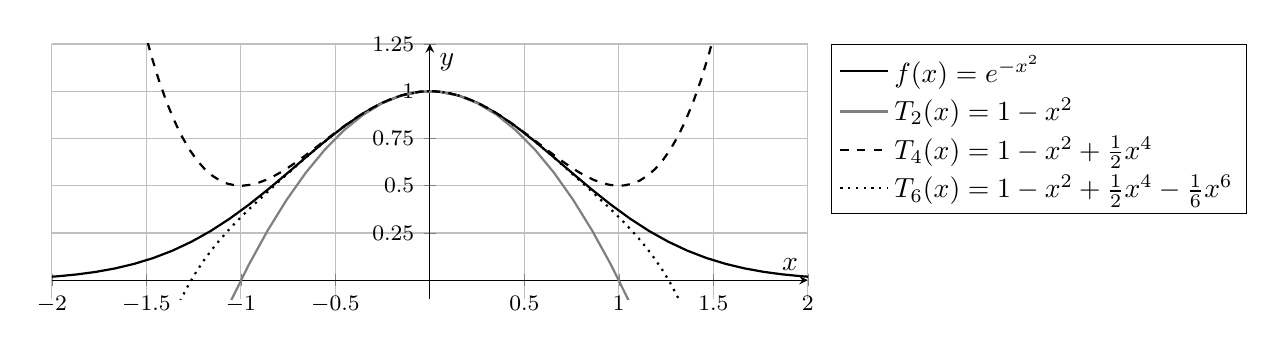
\begin{tikzpicture}
\begin{axis}[
	y=2.4cm,
    x=2.4cm,
	axis x line=middle,
	axis y line = middle,
	ymin=-.1,ymax=1.25,
	xmin=-2,xmax = 2,
    grid=both,
     %xticklabels={\(-\pi\), \( \), ,\( \),\(\pi\)},
%    xtick={-3.14,-1.57,...,3.14},
    ytick={0,.25,...,1.25},
    xlabel=\(x\),
    ylabel=\(y\),
    tick label style={font=\footnotesize},
    legend entries={\(f(x) = e^{-x^2}\),\(T_2(x) = 1-x^2\), \(T_4(x) = 1-x^2 +\tfrac{1}{2}x^4\), \(T_6(x) = 1-x^2 +\tfrac{1}{2}x^4-\tfrac{1}{6}x^6\)},
legend style={nodes=right},
legend pos= outer north east
]

\addplot +[no marks, black, thick,samples = 100] {exp(-x^2)};
\addplot +[no marks, gray, thick, samples = 100] {1-x^2};
\addplot +[no marks, black, thick, dashed, domain=-2:2,samples = 100] {1-x^2+.5*x^4};
\addplot +[no marks, gray, black, dotted, thick, domain=-2:2,samples = 100] {1-x^2+.5*x^4-(x^6)/6};

%\addplot +[no marks, black, thick, samples = 60, domain=-3.14:3.14] {cos(deg(x))};

\end{axis}
\end{tikzpicture}
\end{center}
%\end{minipage}


\begin{enumerate}[a)]


	\item Should you expect \(T_2(0)\) to be a good estimate of \(f(0)\)? Why or why not? 
	
\vspace*{.5in}	
	
	\item Should you expect \(T_2(1)\) to be a good estimate of \(f(1)\)? Why or why not? 
	
\vspace*{.5in}		

\item Use the graph shown above to estimate the accuracy of the approximations:\\
\hfill \(f(1)\approx T_2(1)\), \hfill \(f(1)\approx T_4(1)\), \hfill \(f(1)\approx T_6(1)\) \hfill
	
\vspace*{.75in}		
	
	\item Use the Alternating Series Estimation/Remainder Theorem or Taylor's Formula to estimate the accuracy of the approximations:\\
	 \hfill \(f(1)\approx T_2(1)\), \hfill \(f(1)\approx T_4(1)\), \hfill \(f(1)\approx T_6(1)\) \hfill

\vspace*{.75in}	

\item Finally, we can achieve our goal from the beginning of Chapter 5!  Use \(T_6(x)\) to approximate the area under \(f(x)\) between \(x=0\) and \(x=1\).  Also, explain how to give an estimate of the accuracy of the approximation.
\[
\int_0^1 e^{-x^2}\ dx \approx \int_0^1 T_6(x)\ dx
\]


\end{enumerate}

\vfill



\pagebreak

\item The function \(f(x) = \cos(x)\) is plotted as a solid curve below.\\
Its second degree Maclaurin Polynomial, \(T_2(x) = 1-\frac{x^2}{2}\), is plotted with dashed curve below.


%\begin{minipage}{\textwidth}
\begin{center}
\hspace*{-.75in}
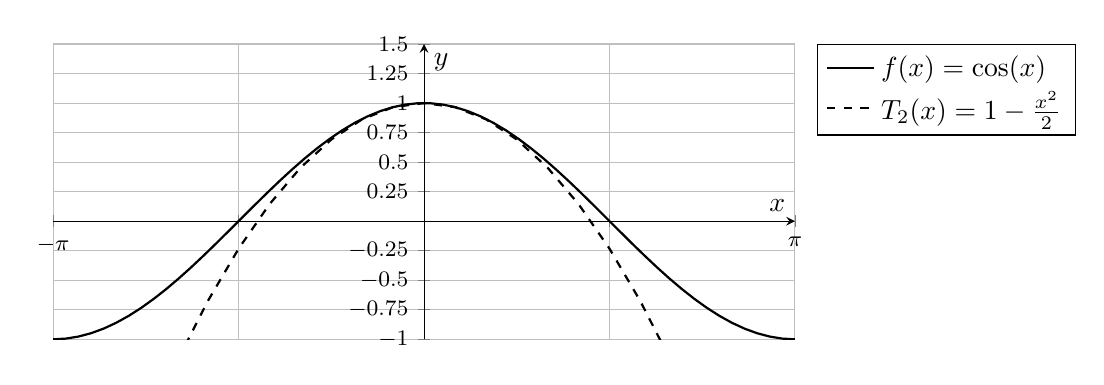
\begin{tikzpicture}
\begin{axis}[
	y=1.5cm,
    x=1.5cm,
	axis x line=middle,
	axis y line = middle,
	ymin=-1,ymax=1.5,
	xmin=-3.14,xmax = 3.14,
    grid=both,
     xticklabels={\(-\pi\), \( \), ,\( \),\(\pi\)},
    xtick={-3.14,-1.57,...,3.14},
    ytick={-1,-.75,...,1.5},
    xlabel=\(x\),
    ylabel=\(y\),
    tick label style={font=\footnotesize},
    legend entries={\(f(x) = \cos(x)\),\(T_2(x) = 1-\tfrac{x^2}{2}\)},
	legend style={nodes=right},
	legend pos= outer north east
]


\addplot +[no marks, black, thick, samples = 60, domain=-3.14:3.14] {cos(deg(x))};
\addplot +[no marks, black, thick, dashed, domain=-3.14:3.14] {1-.5*x^2};

\end{axis}
\end{tikzpicture}
\end{center}
%\end{minipage}


\begin{enumerate}[a)]


	\item Should you expect \(T_2(0)\) to be a good estimate of \(f(0)\)? Why or why not? 
	
\vspace*{.75in}	
	
	\item Should you expect \(T_2(\tfrac{\pi}{2})\) to be a good estimate of \(f(\tfrac{\pi}{2})\)? Why or why not? 
	
\vspace*{.75in}		

\item Use the graph shown above to estimate the accuracy of the approximation \(f(\tfrac{\pi}{2})\approx T_2(\tfrac{\pi}{2})\)
	
\vspace*{.75in}		
	
	\item Use the Alternating Series Estimation Theorem to estimate the accuracy of the approximation \(f(\tfrac{\pi}{2})\approx T_2(\tfrac{\pi}{2})\)


\vspace*{.75in}	

\item Use Taylor's Formula (also known as Lagrange's form of the remainder term) to estimate the accuracy of the approximation \(f(x)\approx T_2(x)\) on the interval \(-\tfrac{\pi}{2} \leq x \leq \tfrac{\pi}{2}\).\\
  \textit{Hint:} Note that for \(f(x) = \cos(x)\),  \(T_2(x) = T_3(x)\), so consider:
\[
R_3(x) = \frac{f^{(4)}(z)}{4!}x^4
\]

\vspace*{.75in}

\end{enumerate}





\end{list}


\end{document}
